% File modified from ugasample.tex and K.M. Walker latex file 
% (Revised 2016 Oct 10)
% Also includes KMW style file which has most AAS symbols

\documentclass[12pt]{report}

% If there are any other \usepackage commands, put them here

\usepackage{setspace}\doublespacing    % important!
\textfloatsep 0.75in                   % important with double spacing
\usepackage[square, numbers, sort&compress]{natbib}
\usepackage{graphicx}
\usepackage[english]{babel}
\usepackage[paperwidth=8.5in,paperheight=11in,bindingoffset=0in,left=1in,right=1in,bottom=1in,top=1in,footskip=0.37in]{geometry}
% \usepackage{physdiss}
\usepackage{caption}
\usepackage{amsmath}
\usepackage{lscape}
\usepackage{longtable}
\usepackage{threeparttable}
\usepackage{amssymb}
\usepackage[stable]{footmisc}
\usepackage{xhfill}
\usepackage[T1]{fontenc}
\usepackage[utf8]{inputenc}
\usepackage{caption}
\usepackage{subcaption}

\captionsetup{belowskip=0pt}

\widowpenalty10000
\clubpenalty10000

\setcounter{secnumdepth}{4} % To number subsubsections 
\newcommand{\ditto}[1][.4pt]{~\textquotedbl~}
\newcommand{\carone}{C~{\footnotesize I}}       % O I
\newcommand{\cartwo}{C~{\footnotesize II}}
\newcommand{\carthree}{C~{\footnotesize III}}    % O~III
\newcommand{\carfour}{C~{\footnotesize IV}}
\newcommand{\carfive}{C~{\footnotesize V}}
\newcommand{\carsix}{C~{\footnotesize VI}}
\newcommand{\carseven}{C~{\footnotesize VII}}
\newcommand{\oxyone}{O~{\footnotesize I}}       % O I
\newcommand{\oxytwo}{O~{\footnotesize II}}
\newcommand{\oxythree}{O~{\footnotesize III}}    % O~III
\newcommand{\oxyfour}{O~{\footnotesize IV}}
\newcommand{\oxyfive}{O~{\footnotesize V}}
\newcommand{\oxysix}{O~{\footnotesize VI}}
\newcommand{\oxyseven}{O~{\footnotesize VII}}
\newcommand{\oxyeight}{O~{\footnotesize VIII}}
\newcommand{\oxynine}{O~{\footnotesize IX}}
\newcommand{\hydone}{H~{\footnotesize I}}
\newcommand{\hydtwo}{H~{\footnotesize II}}
\newcommand{\abundsolar}{$\mathcal{M}_{\sun}$}
\newcommand{\masssol}{$M_{\sun}$}
\newcommand{\abundave}{$\bar{M}$}
\newcommand{\abundscript}{$\mathcal{M}$}
\newcommand{\abundscriptbar}{$\bar{\mathcal{M}}$}
\newcommand{\abundsbarvel}{$\bar{\mathcal{M}_{v}}$}
\newcommand{\superscript}[1]{\ensuremath{^{\textrm{#1}}}}
\newcommand{\subscript}[1]{\ensuremath{_{\textrm{#1}}}}
%\newcommand{\ambfrac}{\ensuremath{\textrm{f}_{\textrm{amb}}}}
\newcommand{\ambfrac}{$f_{amb}$}
\newcommand{\massfrac}{$M_{amb}$}
\newcommand{\scinote}[2]{\ensuremath{{#1}\times10^{#2}}}
%Paper II commands
\newcommand{\simone}{T5r3n3s150} %4.2.1
\newcommand{\simtwo}{T5r3n4s150} %4.2.3
\newcommand{\simthree}{T5r3n3s300} %4.2.4.a
\newcommand{\simfour}{T20r3n3s300} %4.2.4.b
\newcommand{\simfive}{T10r3n3s300} %4.2.4.c
\newcommand{\simsix}{T4r3n3s300} %4.2.4.d
\newcommand{\simseven}{T5r3n4s300} %4.2.6.a
\newcommand{\simeight}{T5r15n4s300} %4.2.6.b
\newcommand{\simnine}{T5r30n4s300} %4.2.6.c
\newcommand{\simmagone}{MHDn3\ensuremath{\perp}} %4.2.5.a
\newcommand{\simmagtwo}{MHDn4\ensuremath{\perp}} %4.2.5.b
\newcommand{\simmagthr}{MHDn4\ensuremath{\parallel}} %4.2.5.c
\newcommand{\simHDone}{HDn3}
\newcommand{\simHDtwo}{HDn4}


\newcommand{\unitkms}{km~s\superscript{-1}}

\newcommand{\majorprof}{William Micheal Dennis} %Major Professor
\newcommand{\proftwo}{Heinz Bernd Schuttler} %Committee Member 1
\newcommand{\profthree}{Micheal Geller} %Committee Member 2
\newcommand{\thesisyear}{2021} % Year of writing the thesis
\newcommand{\yourname}{Dermot (Jim) Heneghan} % Your name as it should appear in the thesis
\newcommand{\thesistitle}{Title of Jim Heneghan's Thesis} % Title of the Thesis
\newcommand{\graddean}{Ron Walcott} % Name of current dean of the graduate school

\graphicspath{{Images/}}
\begin{document}


% Make the official abstract page
\newpage
\pagenumbering{gobble}
\thispagestyle{empty}
\vspace*{18pt}
\begin{center}
\textsc{\thesistitle}\\[18pt]
by\\[18pt]
\textsc{\yourname}\\[12pt]
(Under the Direction of \majorprof)\\[12pt]
\textsc{Abstract}
\end{center}
%Abstract goes here.

% Display the index words (this is a bit fancy):
\begin{list}{\sc Index words:\hfill}{\labelwidth 1.2in\leftmargin 1.4in\labelsep 0.2in}
\item
\begin{flushleft}\singlespacing
Put key words here for future searches. My own dissertation contained the following:
Finite-Difference Time-Domain, 
GPU Acceleration
\end{flushleft}
\end{list}


% Make the official title page
\newpage
\setcounter{page}{1}
\pagenumbering{roman}
\thispagestyle{empty}
\vspace*{18pt}
\begin{center}
\textsc{\thesistitle}\\[18pt]
by\\[18pt]
\textsc{\yourname}\\[12pt]

B.Sc., University of Limerick, 2008\\
M.Sc., University of Limerick, 2011\\
\vfill
A Dissertation Submitted to the Graduate Faculty \\
of The University of Georgia in Partial Fulfillment \\
of the \\
Requirements for the Degree \\[10pt]
\textsc{Doctor of Philosophy}\\[36pt]
\textsc{Athens, Georgia}\\[18pt]
\thesisyear
\end{center}

% Make the copyright page
\newpage
\thispagestyle{empty}
\vspace*{5.5in}
\begin{center}
\copyright~\thesisyear\ \\
\yourname\\
All Rights Reserved
\end{center}

% Make the approval page
\newpage
\thispagestyle{empty}
\vspace*{18pt}
\begin{center}
%\textsc{High Velocity Cloud Interactions With\\ Their Ambient Environment}\\[18pt]
\textsc{\thesistitle}\\[18pt]
by\\[18pt]
\textsc{\yourname}
\end{center}
%\vfill
\vspace*{50pt}
\begin{center}\singlespacing
\hskip 48pt {Approved:}\\
\vskip 12pt
% Two major professors.  If you have only one, change word to "Professor".
\hspace*{155pt}\makebox[100pt][l]{Major Professor:}\majorprof\\
\vskip 12pt
% Committee (use as many lines as needed)
\hspace*{155pt}\makebox[100pt][l]{Committee:       }\proftwo\\
\hspace*{155pt}\makebox[100pt][l]{~                }\profthree        \\
\end{center}
% Approval words - UNCOMMENT AFTER IT HAS BEEN APPROVED
\vfill
\begin{flushleft}\singlespacing
Electronic Version Approved:\\[12pt]
\graddean\\
Dean of the Graduate School\\
The University of Georgia\\
May \thesisyear
\end{flushleft}

% Now we begin the regular LaTeX document.

\chapter*{Dedication}
%chapter* designates a chapter section that is numbered by roman numerals not Arabic numbers


% \pseudochapter{Acknowledgments}
%included in table of contents but no chapter number so use the term \pseudochapter

%\pseudochapter{Preface}
%If your thesis has a preface, this is where it goes.

\tableofcontents % This is filled in later as some command collects the list of Chapters, Sections, Subsections, and more.


\listoftables    % This if filled in later as some command collects the list of tables.
\listoffigures   % This if filled in later as some command collects the list of figures.

\newpage
\pagenumbering{arabic}  % Ordinary pages have Arabic numerals.

%This code is necessary if you want to use indents in paragraphs should be put before begin document
%{
%\raggedright
%\parindent 0.25in
%}


\chapter{Introduction}

   
\section{Chapters}
\label{sec:chap}


% Document Body =========================================================== %
% ------------------------------------------------------------------------- %
\subfile{Chapter2}
\subfile{Chapter3}
% \subfile{subfiles/chapter2}
% \subfile{subfiles/chapter3}
% \subfile{subfiles/chapter4}
% \subfile{subfiles/conclusion}
% ------------------------------------------------------------------------- %
% ========================================================================= %
%%%%%%%%%%%%%%%%%%%%%%%%%%%%%%%%%%%%%%%%%%%%%%%%%%
%%%%%%%%%% Paper I (How to include a chapter that is already published %%%%%%%%%%%%%%
%%%%%%%%%%%%%%%%%%%%%%%%%%%%%%%%%%%%%%%%%%%%%%%%%%
\chapter[An Investigation of the Polariton-Plasmon Coupling in hBN on Nanopatterned Ag Layered Structures]
  {An Investigation of the Polariton-Plasmon Coupling in hBN on Nanopatterned Ag Layered Structures%
  \footnote{D.J.T Heneghan, W. M. Dennis,2021, 
  \emph{Journal TBD}, Vol. TBD, No. TBD. \indent\indent Reprinted here with permission of publisher and authors.}}
  \label{chapter:Ag_hBN}

  \newpage

  \section{Introduction}
  \label{sec:intro}
  	Polaritons are quasiparticles resulting from hybrid modes of photons and charge dipole excitations in crystalline structures \cite{Tolpygo:50}. The two most common types of polaritons are phonon polaritons \cite{Tolpygo:50, Huang:51, Huber:08} and surface plasmon polaritons \cite{Barnes:03}, both of which are relevant to this study. First discovered by Ritchie in 1957 \cite{Ritchie:57}, plasmon-polaritons were observed to propagate along surfaces of conducting thin films \cite{Pines:52}. These surface-plasmon-polaritons (SPPs) remain trapped on the surface due to resonant interactions with the free electrons of the conductor. A unique property of SPPs is that they couple to features within the crystal whose features are smaller than the free space wavelength of the initial coupling photon \cite{Pendry:99}. This confinement of radiation to scales below the diffraction limit has become the primary focus of modern nanophotonics \cite{Caldwell:14}.

    To develop scalable quantum-photonic technologies on-chip integration of the photonic components is required. Such devices have applications in subwavelength imaging \cite{Silva:12,Fang:05}, biosensing \cite{Kneipp:97, Talley:05, Rodrigo:15}, thin film sensing \cite{Fali:19} and quantum information \cite{Chang:06, Gonzalez-Tudela:11, Bhimanapati:15}. After it’s discovery much interest was shown in the study of graphene as a medium for tunable photon-plasmon coupling at the mid-infrared range \cite{Koppens:11}. However, in the second decade of this century there has been a rapidly increasing number of papers in the study of non-graphene two dimensional materials \cite{Bhimanapati:15}. In 2014 Dai \textit{et al}. demonstrated higher confinement within hexagonal boron nitride (hBN) with lower losses than graphene SPPs \cite{Dai:14} and a strong confinement regime up to $\rm \lambda 86$ \cite{Caldwell:14}. This advantageous property is due to the hyperbolic nature of hBN’s permittivity tensor which contains oppositely signed principle components within the mid-infrared range \cite{Kumar:15}. While other artificial hyperbolic materials have been demonstrated, they suffer from higher losses and increased fabrication costs in comparison to natural hBN \cite{Biehs:12, Guo:12, Cortes:12}. Since hBN SPPs reside in a similar mid-infrared regime as graphene’s, hBN has the potential to be used in similar devices to those fabricated using graphene such as solar panels \cite{Bonaccorso:10}. While hBN’s ability to endure temperatures up to 1773 K makes it a versatile material for high temperature applications \cite{Jacob:12, Liu:07}. This shared absorptance range also allows for graphene-hBN hetero-devices \cite{Kretinin:14, Dean:10}. Proximity effects due to layered hBN-graphene interactions has been shown to lead to the formation of secondary Dirac points\cite{Dean:13, Hunt:13, Yu:14}. Such properties are of use for breaking of time-reversal-symmetry \cite{Haldane:08, Raghu:08, Chen:19}, enabling the study of the quantum Hall effect \cite{Dean:13, Hunt:13, Yu:14}, tunable superconductivity \cite{Chen:19}, and topological currents and states \cite{Chen:20, Novoselov:16}. Graphene’s high tunability to allows such devices to couple into a greater spectral range, while hBN’s higher quality factor to transport SPPs at a higher efficiency with low levels of damping \cite{Kumar:15, Dean:10, Geim:13, Woessner:15}. However, the plasmon losses due to electron scattering by thermal phonons it is necessary to reduce dielectric losses by reducing damping \cite{Woessner:15}.

    One such solution for reducing this dielectric loss is to use a hetero device that incorporates a metallic diffraction grating underneath a hBN layer. Zhao and Zhang demonstrated near-perfect absorptance in hBN/metal gratings due to hyperbolic phonon-plasmon polariton coupling \cite{Zhao:17}. Recently Yang \textit{et al}.\cite{Yang:20} reported the coupling of phonon-polaritons between a hexagonal pattern of circular cavities in $\rm SiO_{2}$. The experimental observations in this work used a diffraction grating constructed of a hexagonal pattern of holes in an Ag film under an 80 nm thick layer of hBN and over a Si substrate. Up until recently it has been difficult to observe many of the finer near field spectral features of hBN devices due to lack of access to powerful broadband IR laser sources to effectively couple with optical phonons \cite{Yang:20, Alfaro-Mozaz:17, Autore:18}. Recent work has shown scattering-type scanning near-field optical microscopy (s-SNOM) to be a powerful tool to observe, manipulate and quantify polariton coupling in hBN based heterostructures \cite{Fali:19, Folland:18}. Related studies investigating phonon-plasmon coupling using Fourier-transform infrared (FTIR) spectroscopy have been performed on polymethyl methacrylate (PMMA) \cite{Cheng:15, Wan:16}. The results reported here involved a coupled experimental/simulational study of an hBN hetero device. The device is an hBN film atop of nanopatternerned (hexagonal pattern of circular holes) silver (Ag) film deposited on a silicon (Si) substrate.

    Computer simulations were performed using an in-house Finite-Difference Time-Domain (FDTD) code. FDTD is a technique for simulating electrodynamic systems by numerically integrating the Maxwell curl equations by using a finite-difference approximation. Initially proposed by Yee in 1966 \cite{Kane:66} the popularity of the method has grown in parallel to the advances in computing over the last nine decades. The time-domain nature of FDTD means that several frequencies of interest can be studied from a single simulation by using a broadband source. FDTD gives us control over the parameter space to simulate a range of possible device specifications including grating pitch length, film thickness and hole size.

    Due to the large time constants of the hBN and Ag films which comprised the devices studied in this investigation, $\rm \geq 2 \times 106$ time steps time steps were needed for each simulation. This necessitated incorporating GPU acceleration into the inhouse code to greatly reduce the runtime required.

    The FDTD simulations reported in this paper enable not only direct comparison with experimental s-SNOM images, but also can provide detailed three-dimensional spatial information on the vector components of the electric fields within the device, information on plasmon-polariton coupling and allow the polariton wavelength to be unambiguously extracted.

  \section{Results and Discussion}
  \label{sec:RnD}
    Electromagnetic simulations were performed using the Finite-Difference Time-Domain (FDTD) method    \cite{Kane:66} using an in-house designed code. The FDTD method numerically integrates the Maxwell curl equations with second-order accuracy as detailed in Ref. \cite{Taflove:05}.

      \begin{figure}[h]
        \centering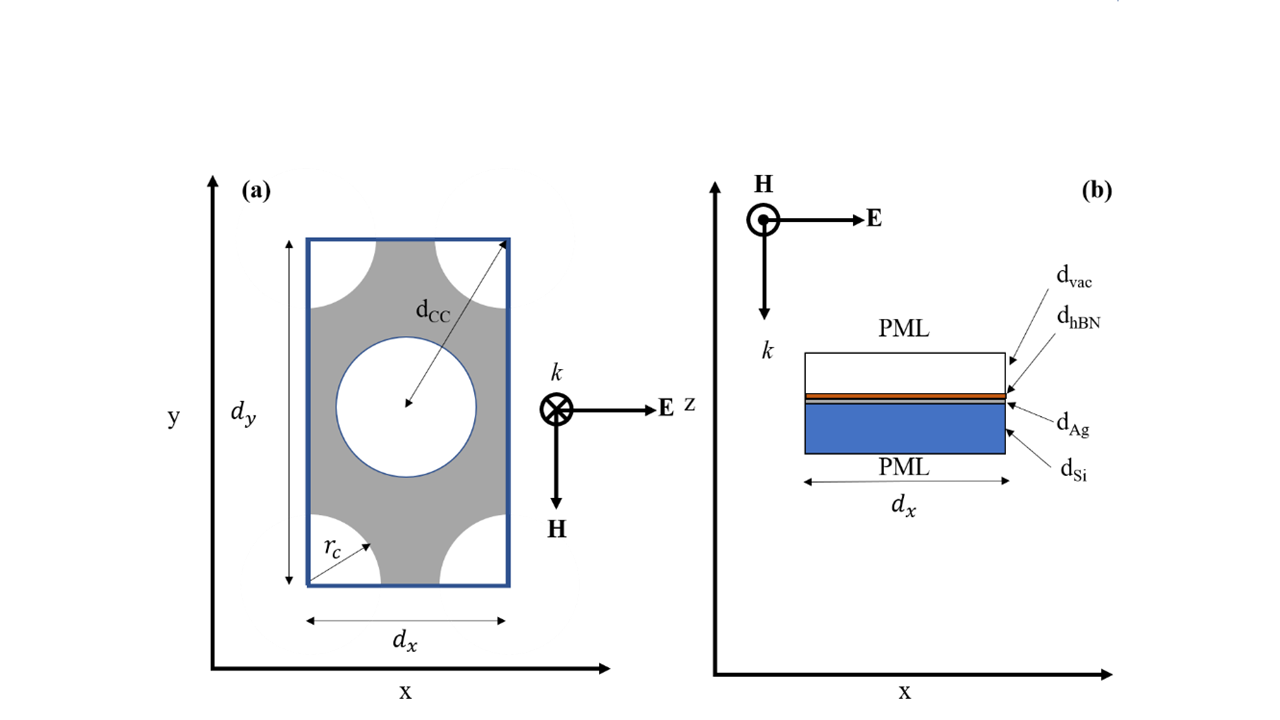
\includegraphics[width=0.9\textwidth]{FiguresCh4/StructurehBNAgHex.png}
        \caption{Simulational structure.}
        \caption*{Schematic of the hBN/Ag structure simulated on this work. \textbf{(a)} Plane view at the hBN/Ag interface. The symmetry reduced unit cell is outlined in red. \textbf{(b)} Cross-sectional view. CPML: Convolutional perfectly matched layer boundary conditions terminated the z direction boundaries. Periodic boundary conditions terminated the x and y boundaries. The unit cell lengths in the x- and y- directions are $d_{x} $ and $d_{y}$, respectively. The layer thicknesses beyond the CPMLs were $d_{\rm{VAC}} = 0.87$ $\rm \mu$m, $d_{\rm{hBN}} = 80$ nm, $d_{\rm{Si}} = 1.0$ $\rm \mu$m, $d_{\rm{Ag}} = 50$ nm. The radius of the holes is $r_{C} = 0.68$ $\rm \mu$m. The distance between the centers of the cylindrical holes is $d_{CC} = d_{x} $. The directions of the \textbf{\textit{E}}-field, \textbf{\textit{H}}-Field and propagation vector \textbf{\textit{k}} is shown in both panes.}
        \label{fig:1}
      \end{figure}

    The details of the nanopatterned structure simulated in this work are shown in Figure ~\ref{fig:1}. The structure comprised of an 80 nm sheet of hexagonal boron nitride (hBN) deposited on a 50 nm thick film of nanopatterned Ag atop of a Si substrate. The Ag film was patterned with circular holes of radius 0.68 $\rm \mu m$ arranged in a hexagonal lattice with a distance between the centers of $\rm d_{CC}$, which was varied during this work.

    In order to decrease the runtime of the simulations GPU acceleration was used. A combination of OpenACC and CUDA \cite{PGI:20} methodologies enabled the simulations to be sped up by a factor of 70. This enabled higher resolution simulations to be performed in the allowed timeframe.

    For all simulations performed a broadband, plane wave source was used. The time profile of the source was a Ricker wavelet \cite{Ricker:43} centered on 1667 $\rm cm^{-1} (6  \mu m$). This source injects a laterally uniform in time pulse using the total-field scattered-field (TFSF) interface \cite{Merewether:80}. The source was x-polarized and propagated in the negative z-direction. The use of the TFSF method enabled sensors to be placed above the TFSF boundary in order to record only the reflected field values.
    
    To prevent divergence in the simulation caused by the patterned Ag layer a convolutional perfectly matched layer (CPML) \cite{Gvozdic:17} boundary was used as the CPML has been shown to be more stable than a uniaxial perfectly matching layer (UPML) \cite{Sacks:95} absorbing boundary for simulations of this kind. Periodic boundary conditions are used in the transverse directions. In the positive and negative z-directions, the simulation was terminated by 50 perfectly matched layers. Due to the difference between the length scales of features in the transverse and longitudinal directions, the computational grid used cell sizes in the ratio of 10:10:1 in the x-, y- and z-dimensions, respectively. The resonance frequency of the patterned Ag layer was found to be sensitive to the spatial resolution used in the simulation, so convergence testing was performed, and a working resolution of $\rm \Delta x = 20 \  nm, \ \Delta y = \ 20 \ nm, \ \Delta z = 2 \ nm$ was selected to be a good compromise between simulation accuracy and runtime.

    Reflectance and transmittance spectra were calculated using a transverse wave vector expansion method from calculations performed by signal monitors during the simulation. Each of these monitors was a two-dimensional plane which calculated the discrete Fourier-transform (DFT) for the wavelengths of interest for every grid point within the monitor’s cross-sectional plane. The monitor performed this function for each of the three electric field components. The incidence data required to normalize the results were also calculated by DFT during the TFSF update step.

    For direct comparison with the experimental imaging data, the spectrally resolved (using DFT) electric field as a function of position was exported from a sensor located on a plane at the hBN/vacuum interface. This data was visualized using a color map. The polariton wavelength could be extracted from the above data as discussed in this report and further detailed in the supplemental materials for direct comparison with experiment.

    The various components of the device were modelled as follows. The Si substrate was simulated using a simple dielectric with $\rm \varepsilon_{r}=11.7$. The Ag film was simulated using wavelength dependent refractive index data as detailed in the Handbook of Optical Constants of Solids I-III \cite{Palik:85} to fit to a Debye/Drude model. The hBN layer was simulated using a Lorentz model. i.e.,

          \begin{equation*}
            \overleftrightarrow{\varepsilon} = \begin{pmatrix} \varepsilon_{x}&0&0\\
                                          0&\varepsilon_{y}&0\\
                                          0&0&\varepsilon_{z}\end{pmatrix}
          \end{equation*}
          \\

    where $\varepsilon_{k}(\infty)$ is the \textit{kth} component (where \textit{k=x,y,z}) of the dielectric function at infinity, $\omega_{k} $ is the frequency of a transverse optical phonon propagating in the \textit{kth} direction, the factor $S_{k} \omega_{k}^{2} $ can be written in the form $\varepsilon_{k}(\infty)(\omega_{\rm{LO}}^{2} - \omega_{\rm{TO}}^{2}) $  \cite{Kumar:15}, showing the explicit dependence on the longitudinal optical (LO) and transverse optical (TO) phonon frequencies. Given the polarization of the excitation source (see Figure 1) the in-plane parameters used in this research were $\varepsilon_{x,y}(\infty)= \rm{4.87}, S_{x,y} = \rm{0.61}, \hbar \omega_{x,y} = $ 170.1 meV. The out-of-plane parameters were  $\varepsilon_{z}(\infty)= \rm{2.95}, \ S_{z} = \rm{0.61}, \ \gamma_{z} = $ 0.25 meV, and $\hbar \omega_{z} = $ 92.5 meV from ref. \cite{Jiang:18}. The notable exception was the planar damping constant $\gamma_{x,y} $, which has been shown to have a strong thickness dependence by Caldwell \textit{et al}. \cite{Caldwell:14}. Using results from the Caldwell group, as detailed in the supplemental materials section, the appropriate value of $\gamma_{x,y} $ for a of film thickness 83 nm was found to be 3.97 meV. For implementation in the FDTD method, finite-difference approximations were obtained by converting the respective frequency domain permittivity tensors to the time domain using the Z-transform method \cite{Sullivan:96, Sakurai:17}.
    \\

      \begin{figure}[!htb]
        \centering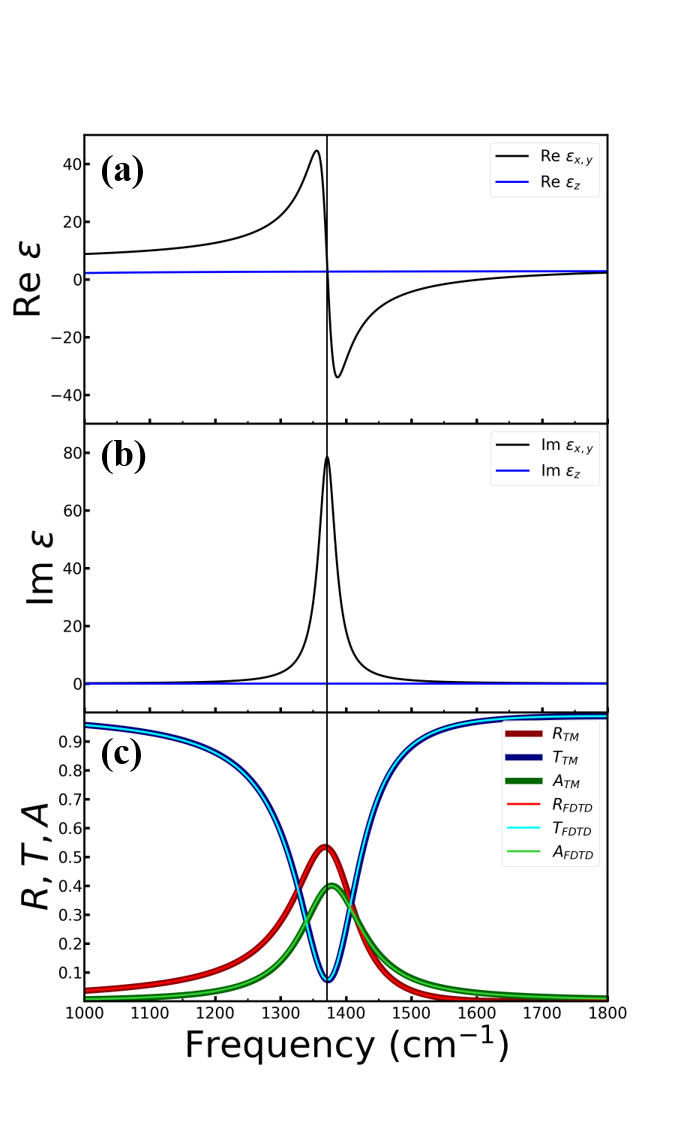
\includegraphics[width=0.5\textwidth]{Mar5DisserrtationPics/Fig2.png}
        \caption{Dielectric function and resulting spectra of 80 nm hBN.}
        \caption*{\textbf{(a)} Real part of $\varepsilon_{x,y}$ (black) and $\varepsilon_{z}$ (blue) for hBN. \textbf{(b)} Imaginary part of $\varepsilon_{x,y}$ (black) and $\varepsilon_{z}$ (blue) for hBN. The vertical line in this figure indicates the peak of Im $\varepsilon_{x,y}$ \textbf{(c)}Plot of reflectance (R), transmittance (T) and absorptance (A) for an 80 nm thin film of hBN in vacuum as calculated using both the transfer matrix and FDTD methods. The peak in absorptance occurs at 1377 $\rm cm^{-1}$.}
        \label{fig:2}
      \end{figure}

    Figure ~\ref{fig:2} (a) and (b) shows the frequency dependence of the real and imaginary components of the dielectric tensor for an hBN film with a thickness of dhBN = 80 nm suspended in vacuum. Figure ~\ref{fig:2} (c) shows the normal incidence reflectance, transmittance, and absorptance spectra for this film calculated using the both the transfer matrix method and the FDTD method as detailed below. Frequency domain data was recorded in the FDTD simulations using the aforementioned DFT sensors. These sensors recorded the reflected and transmitted field data while a separate sensor within the TFSF source function recorded incident field data. This data was then used to calculate the ratio of reflected/transmitted and incident signal as a function of frequency. For the simulation in Figure ~\ref{fig:2} (c) these sensors were placed at z = 0.01 $\rm \mu$m and z = 1.98 $\rm \mu$m. The absorptance (A) spectrum for the film was calculated using A = 1 – (T + R) where the reflectance (R) and transmittance (T) spectra were calculated using DFT sensors.
    \\

      \begin{figure}[!htb]
        \centering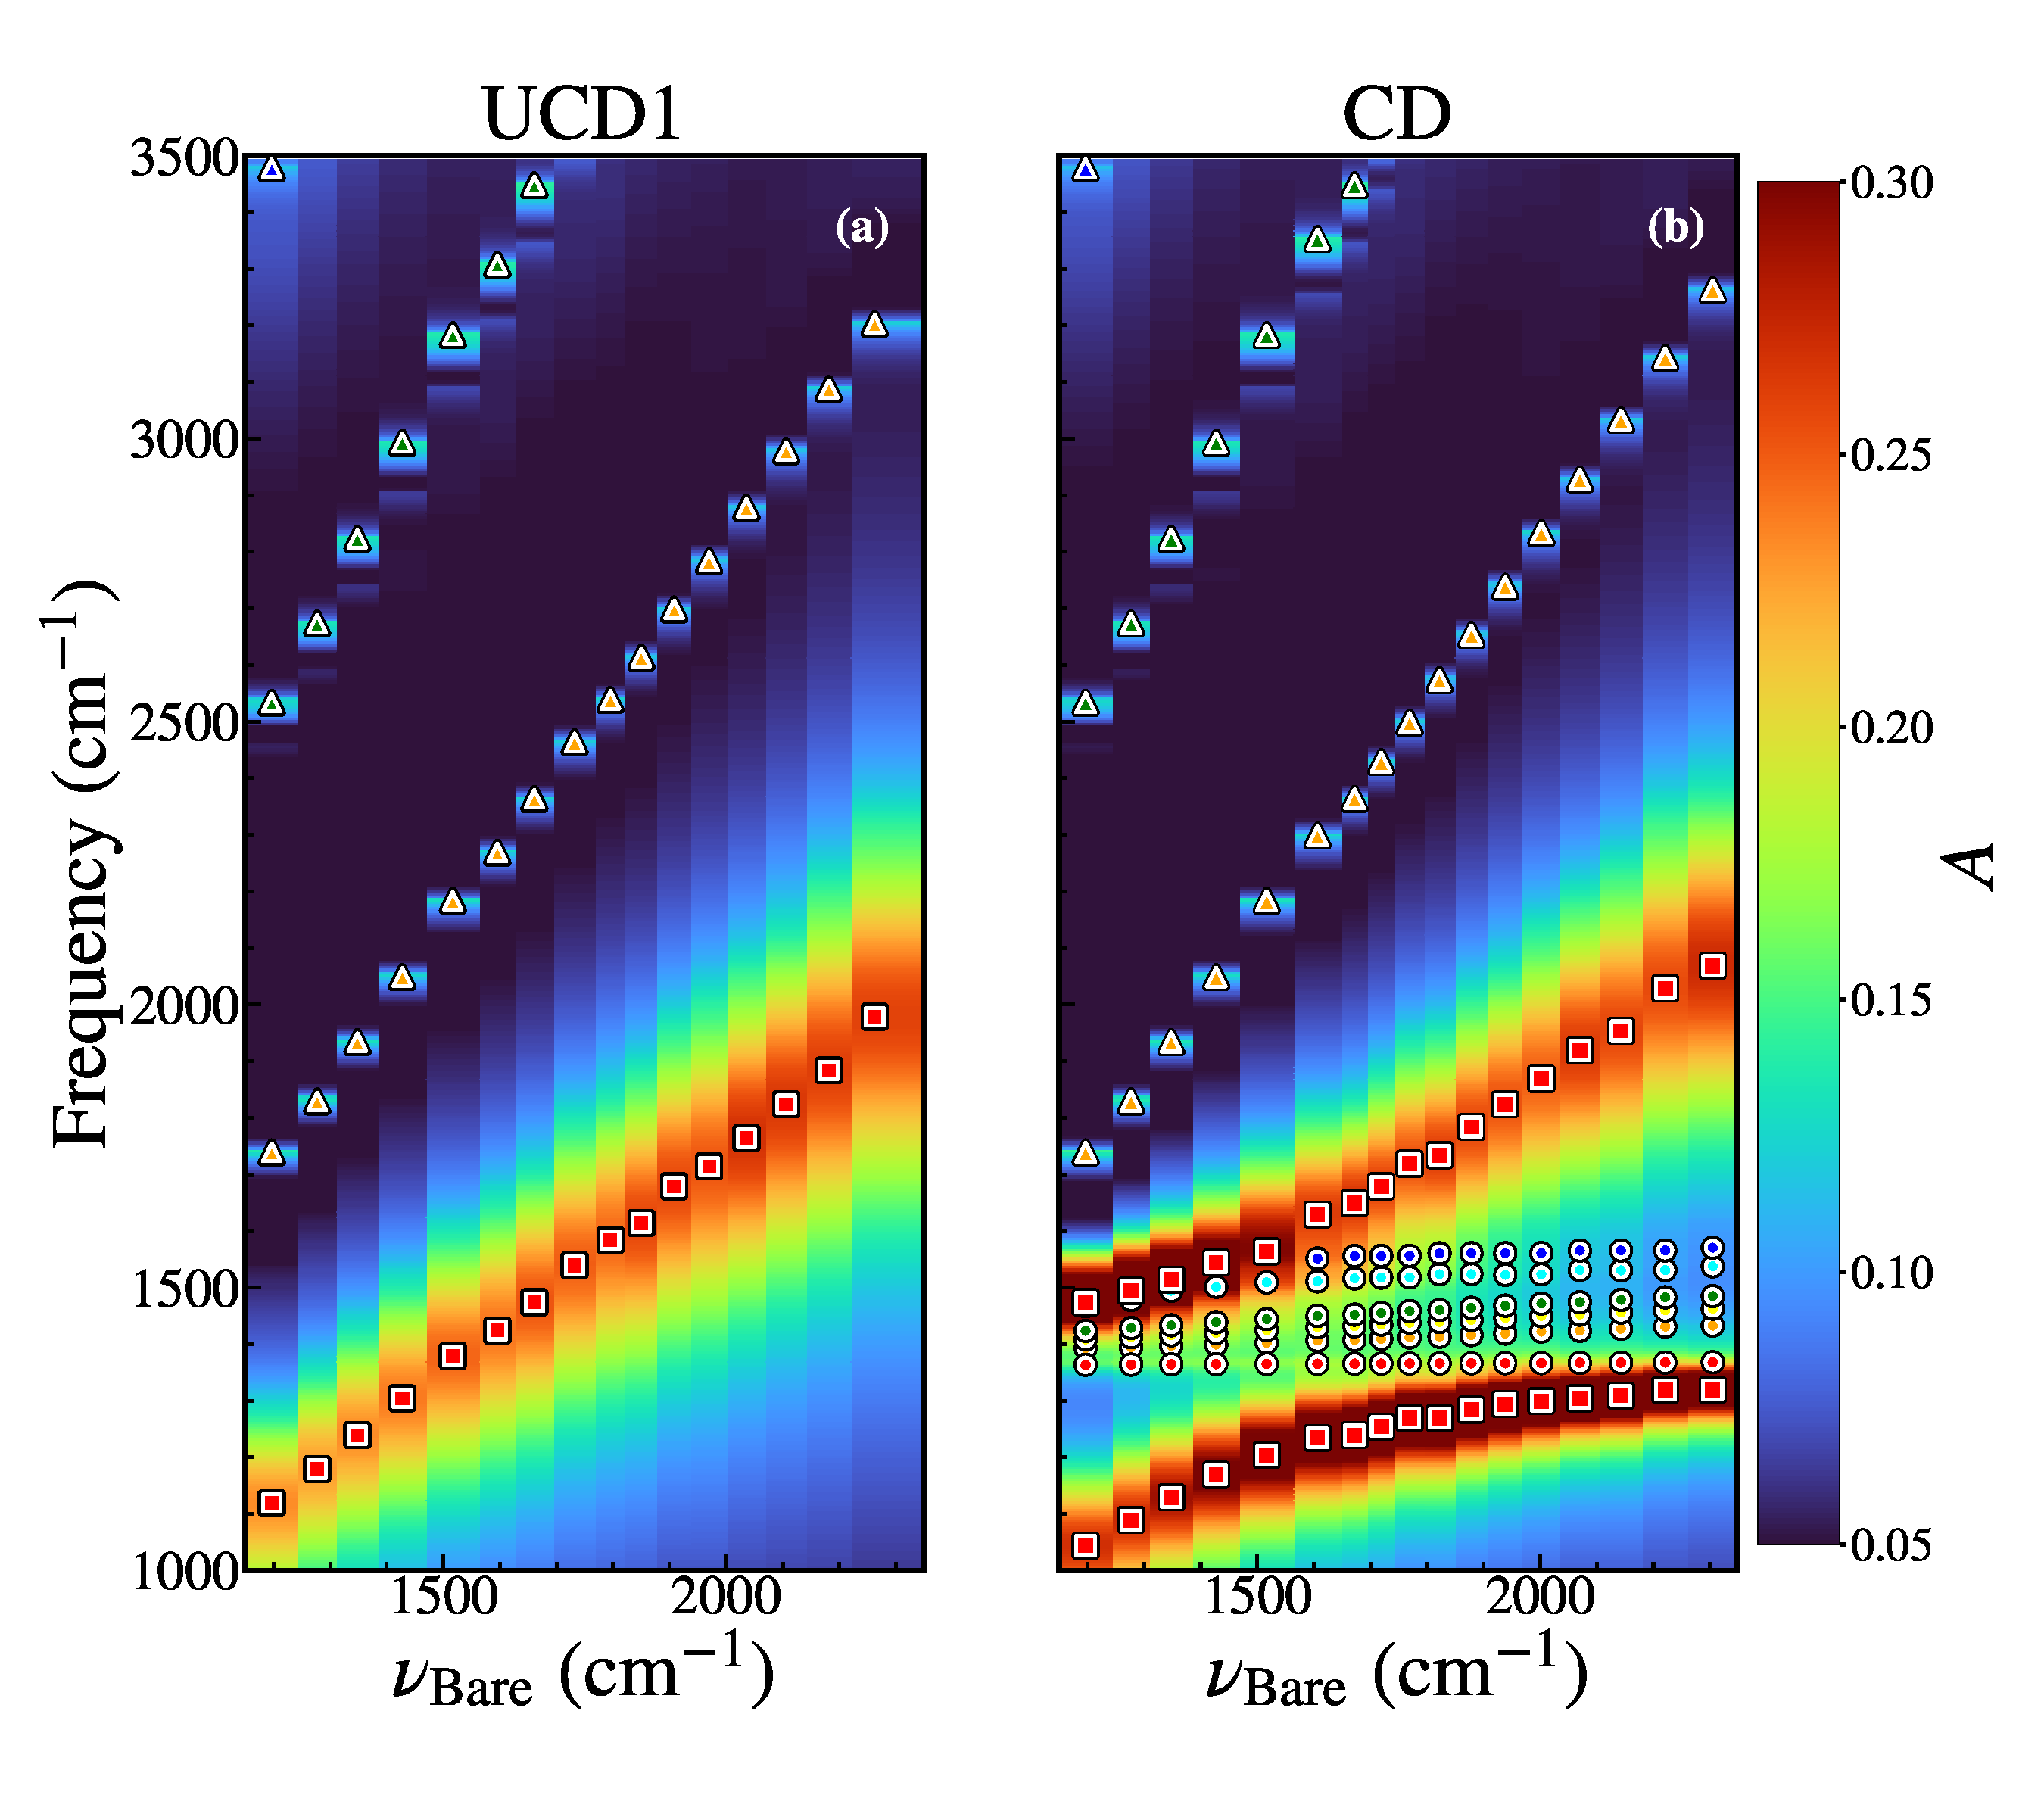
\includegraphics[width=0.5\textwidth]{Mar5DisserrtationPics/Fig3.png}
        \caption{Absorptance spectra for devices simulated.}
        \caption*{\textbf{(a)} The absorptance spectrum of the bare nanopatterned Ag on Si device as function of $d_{CC}$. \textbf{(b)} The absorptance spectra of devices with an uncoupled anisotropic dielectric layer on top of the structures depicted in \textbf{(a)}. \textbf{(c)} The absorptance spectra of devices with an hBN (coupled) layer on structures depicted in \textbf{(a)}. The vertical black line in this figure indicates the absorption peak that was observed for the 80 nm thick layer of hBN in vacuum shown in Figure ~\ref{fig:2}.}
        \label{fig:3}
      \end{figure}

    In order to ensure resonance between the polaritons supported by the hBN layer and the plasmons supported by the nanopatterned Ag/Si structure (bare device). A series of FDTD simulations were performed at range of distances between the centers of the holes ($d_{CC}$). The absorptance spectrum for each of the structures was calculated as described above. As the value of $d_{CC}$ was increased, a red shift in the absorptance spectrum was observed, as shown in Figure ~\ref{fig:3} (a). This observation enabled the absorptance resonance of the bare device to be tuned to close the resonance observed in Figure ~\ref{fig:2} (c) for an 80 nm thick layer of hBN. Following the approach of Wan \textit{et al}. \cite{Wan:16}, the properties of a second series of devices (uncoupled devices) with a nonresonant dielectric layer on top of the nanopatterned Ag/Si structure (bare device) are also investigated. Specifically, for these devices, the top layer is an anisotropic dielectric with $\varepsilon_{x,y}(\infty)= \rm{4.87}$ and $\varepsilon_{z}(\infty)= \rm{2.95}$, respectively (i.e., $\varepsilon_{x,y}(\infty)$ and $\varepsilon_{z}(\infty)$ for hBN, respectively). The absorptance spectra for the uncoupled devices are shown in Figure ~\ref{fig:3} (b). The peaks of the uncoupled device absorptance spectra are slightly red-shifted compared to the peaks of the bare device absorption spectra. The uncoupled device with an absorptance peak that is most resonant with the hBN absorption peak is the device with $d_{CC}$ = 2.38 $\rm \mu$m. The final series of devices (coupled devices), comprising an 80 nm thick hBN layer on top of the bare devices. The absorptance of the coupled devices are shown in Figure  ~\ref{fig:3} (c). In this case the absorptance spectra splits into two major peaks, the positions of which vary with $d_{CC}$ or equivalently with the frequency ($\nu_{\rm{bare}}$) of the peak absorptance of the bare device. In addition, there is a smaller peak at 1468 $\rm cm^{-1}$ the position of which is independent of $d_{CC}(\nu_{\rm{bare}})$, it is notable that this peak occurs in the spectral region where Re $\varepsilon_{x,y}$ is strongly negative.

      \begin{figure}[!htb]
        \centering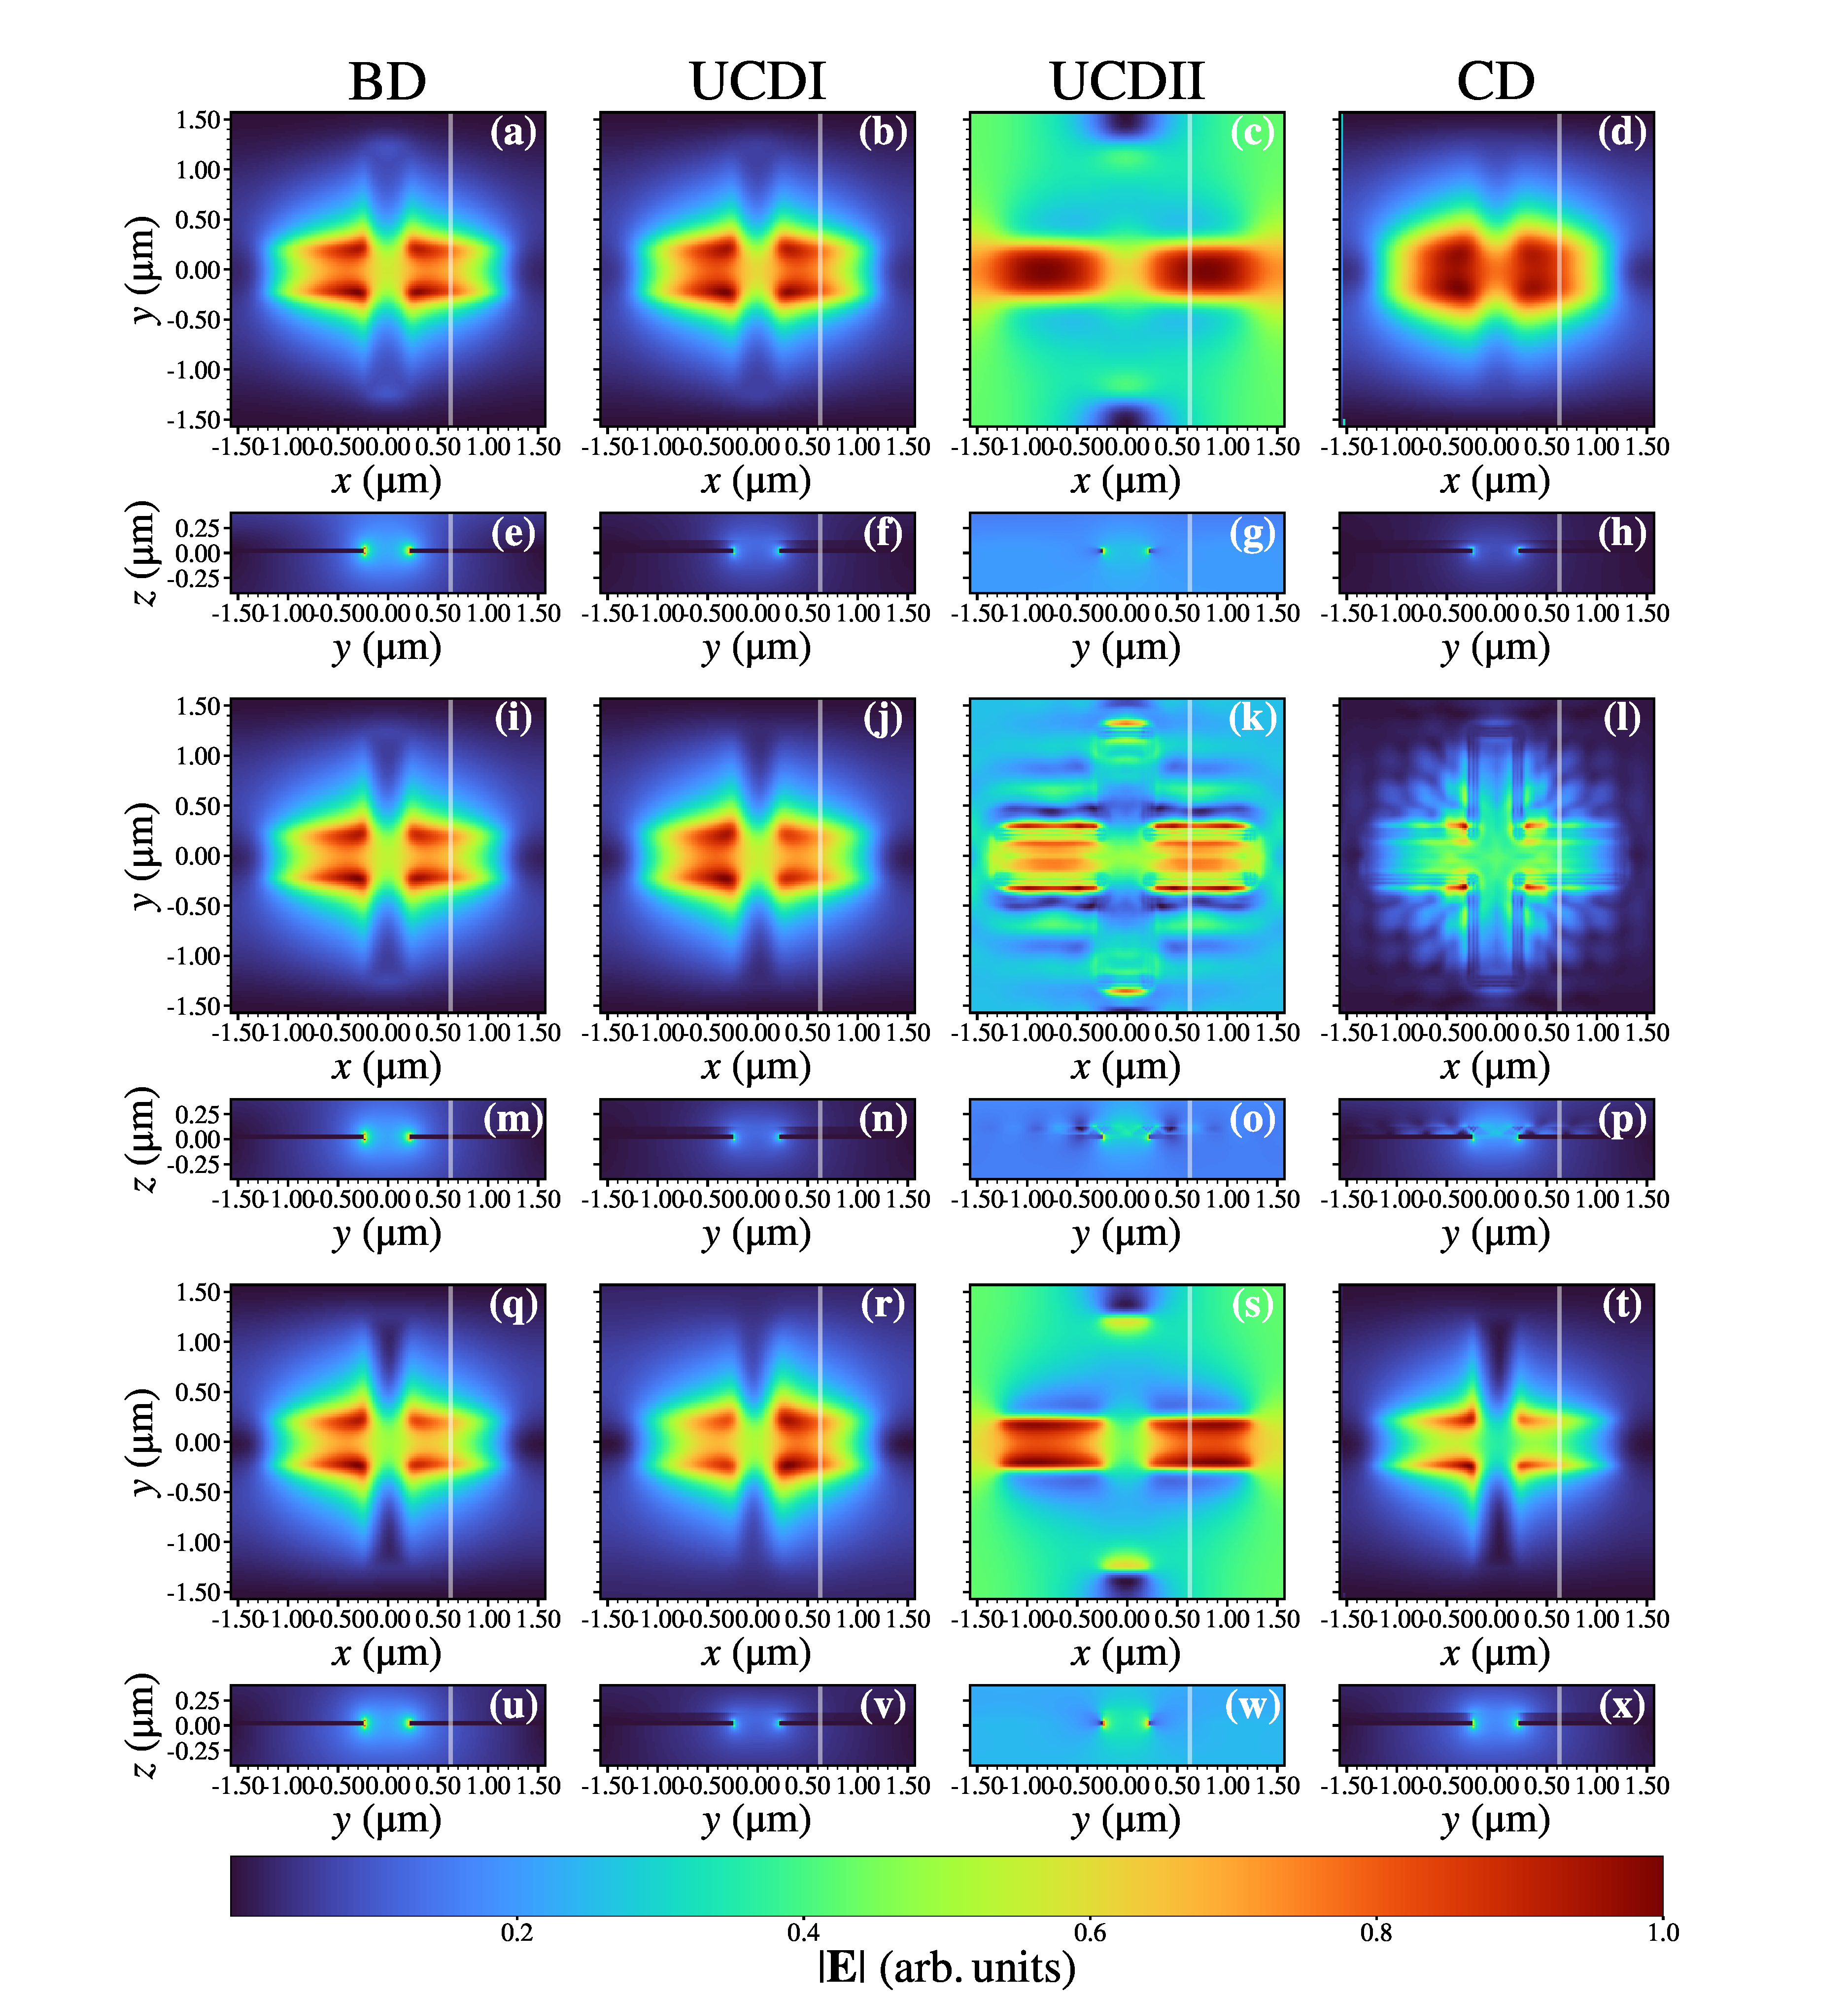
\includegraphics[width=0.95\textwidth]{Mar5DisserrtationPics/Fig4.png}
        \caption{Rasterized frequency "heat maps" for coupled and uncoupled devices}
        \caption*{\textbf{(a)} Absorptance spectra for the uncoupled devices vs the peak frequency of the bare device. The symbols indicate the peak in the absorptance spectra of each uncoupled device and clear show the tuning of the plasmon resonance as function of $d_{CC}$. \textbf{(b)} The absorptance spectra for the hBN (coupled) device. The symbols indicate the peaks in the absorptance spectra and clearly show the coupling between the plasmonic resonance and the hBN TO phonon mode.}
        \label{fig:4}
      \end{figure}

    In order to better analyze the absorptance peak frequency shifts observed in Figure ~\ref{fig:3}, the data in Figure ~\ref{fig:3}(b) and (c) were plotted in colormap form as a function of $\nu_{\rm{bare}}$ in Figure ~\ref{fig:4}(a) and ~\ref{fig:4} (b) respectively. The peak positions were calculated as detailed in the supplemental materials and plotted on top of the colormaps as prescribed in \cite{Wan:16}. Analogously to the reflection data of Wan et al. \cite{Wan:16}, the plasmon peak in the uncoupled device tracks linearly with $\nu_{\rm{bare}}$, while the absorptance peaks of the coupled device open up a small gap and splits into upper and lower branches. For the coupled device with $d_{CC}$ = 2.38 $\rm \mu$m, the difference in frequency between the peaks in absorption is $\Omega$ = 89.7 $\rm cm^{-1}$, which interestingly is close to the range of values, $\Omega$ = 63.4 – 86.7 $\rm cm^{-1}$, reported by Wan et al. for the PMMA/gold meta material structures with PMMA thicknesses ranging from 40 – 100 $\rm \mu$m. Application of degenerate perturbation theory \cite{Sakurai:17} applied to this two-level system enabled the phonon-plasmon coupling strength $\Delta_{PP} = \rm  \Omega = 89.7 cm^{-1}$ to be extracted.

    Figure ~\ref{fig:5} shows components and magnitude of the electric field in a cross-section through center of both the coupled and uncoupled devices with $d_{CC}$  = 2.38 $\rm \mu$m. Data for devices with other values of $d_{CC}$  are presented in the supplemental materials. The fieldmaps shown in Figure ~\ref{fig:5} are four of the frequencies of interest that were monitored within the hBN absorptance peak in Figure ~\ref{fig:2}(c), namely $\nu$ = 1299, 1361, 1471, and 1538 $\rm cm^{-1}$. By comparing the field maps of the coupled and uncoupled devices, it is possible to isolate the behavior associated with the hBN TO phonon mode. At $\nu$ = 1299 $\rm cm^{-1}$ the field maps for the both the coupled and uncoupled devices are very similar indicating that at this frequency the behavior of the coupled device is predominantly plasmonic. At $\nu$ = 1361 $\rm cm^{-1}$, which is the lowest frequency point of upper branch in Figure ~\ref{fig:5} (b) and is close in frequency to the peak of the hBN in vacuum absorptance band in Figure ~\ref{fig:2} (c), the data in the coupled device appears to be predominantly plasmonic but the fields are confined in the region of the Ag and hBN layers. At $\nu$ = 1471 $\rm cm^{-1}$, which is in the vicinity of the small fixed frequency absorptance peak in Figure ~\ref{fig:2} (c), field maps for the both the coupled and uncoupled devices are very different indicating that at this frequency the behavior of the coupled device is predominantly due to the hBN TO phonon. It is notable that in this region the electric field is strongly confined to and appears to be guided within the hBN layer. Finally, at $\nu$ = 1538 $\rm cm^{-1}$, the field maps for both the coupled and uncoupled devices are also very different indicating that at this frequency the behavior of the coupled device is predominantly due to the hBN TO phonon.

    It is not immediately obvious how to extract the polariton wavelength ($\lambda_{P}$) from the above data, in particular the absolute value field data which is directly comparable to experiment. This is due in part not only to the variety and complexity of the mode structure but also due to a non-zero background contribution (see for example, the x-polarized data for the coupled devices in Figure ~\ref{fig:5}). Fortunately, the y-polarized data is comparatively background free showing an alternating field pattern from which the phonon wavelength may be extracted. The y-polarized data was analyzed in the spectral region 1466 – 1570 $\rm cm^{-1}$ and where possible, the distance between successive peaks was averaged (as described in the supplemental materials) in two regions: (a) In the region where the hBN layer was supported by Ag (denoted Vacuum|hBN|Ag) and (b) where the hBN was over one of the circular holes in the Ag film (denoted Vacuum|hBN|Vacuum). In the Vacuum|hBN|Ag case phonon wavelengths in the range $\lambda_{P}$ = 0.16 – 0.33 $\rm \mu$m were extracted. In the Vacuum|hBN|Vacuum case phonon wavelengths in the range $\lambda_{P}$ = 0.40 – 0.70 $\rm \mu$m were extracted. The above values of $\lambda_{P}$ were compared with phonon-polariton dispersion curves calculated using formalism described in [20] for (a) an 80 nm layer of hBN in the Vacuum|hBN|Ag configurationand (b) the Vacuum|hBN|Vacuum configuration. The phonon-polariton wavelengths calculated above were both found to lie close to the expected dispersion curves for the cases (a) and (b) above. There was one notable exception to the data described above. The value of $\lambda_{P}$ = 0.28 $\rm \mu$m for the Vacuum|hBN|Vacuum case monitored at frequencies in the vicinity of $\nu$ = 1466 $\rm cm^{-1}$ was much shorter than expected value of 2.1 $\rm \mu$m indicating that the field variation observed in this case is not solely due to the phonon-polariton, but is caused by some other effect, possibly strong confinement and guiding in the hBN layer.

      \begin{figure}[!htb]
        \centering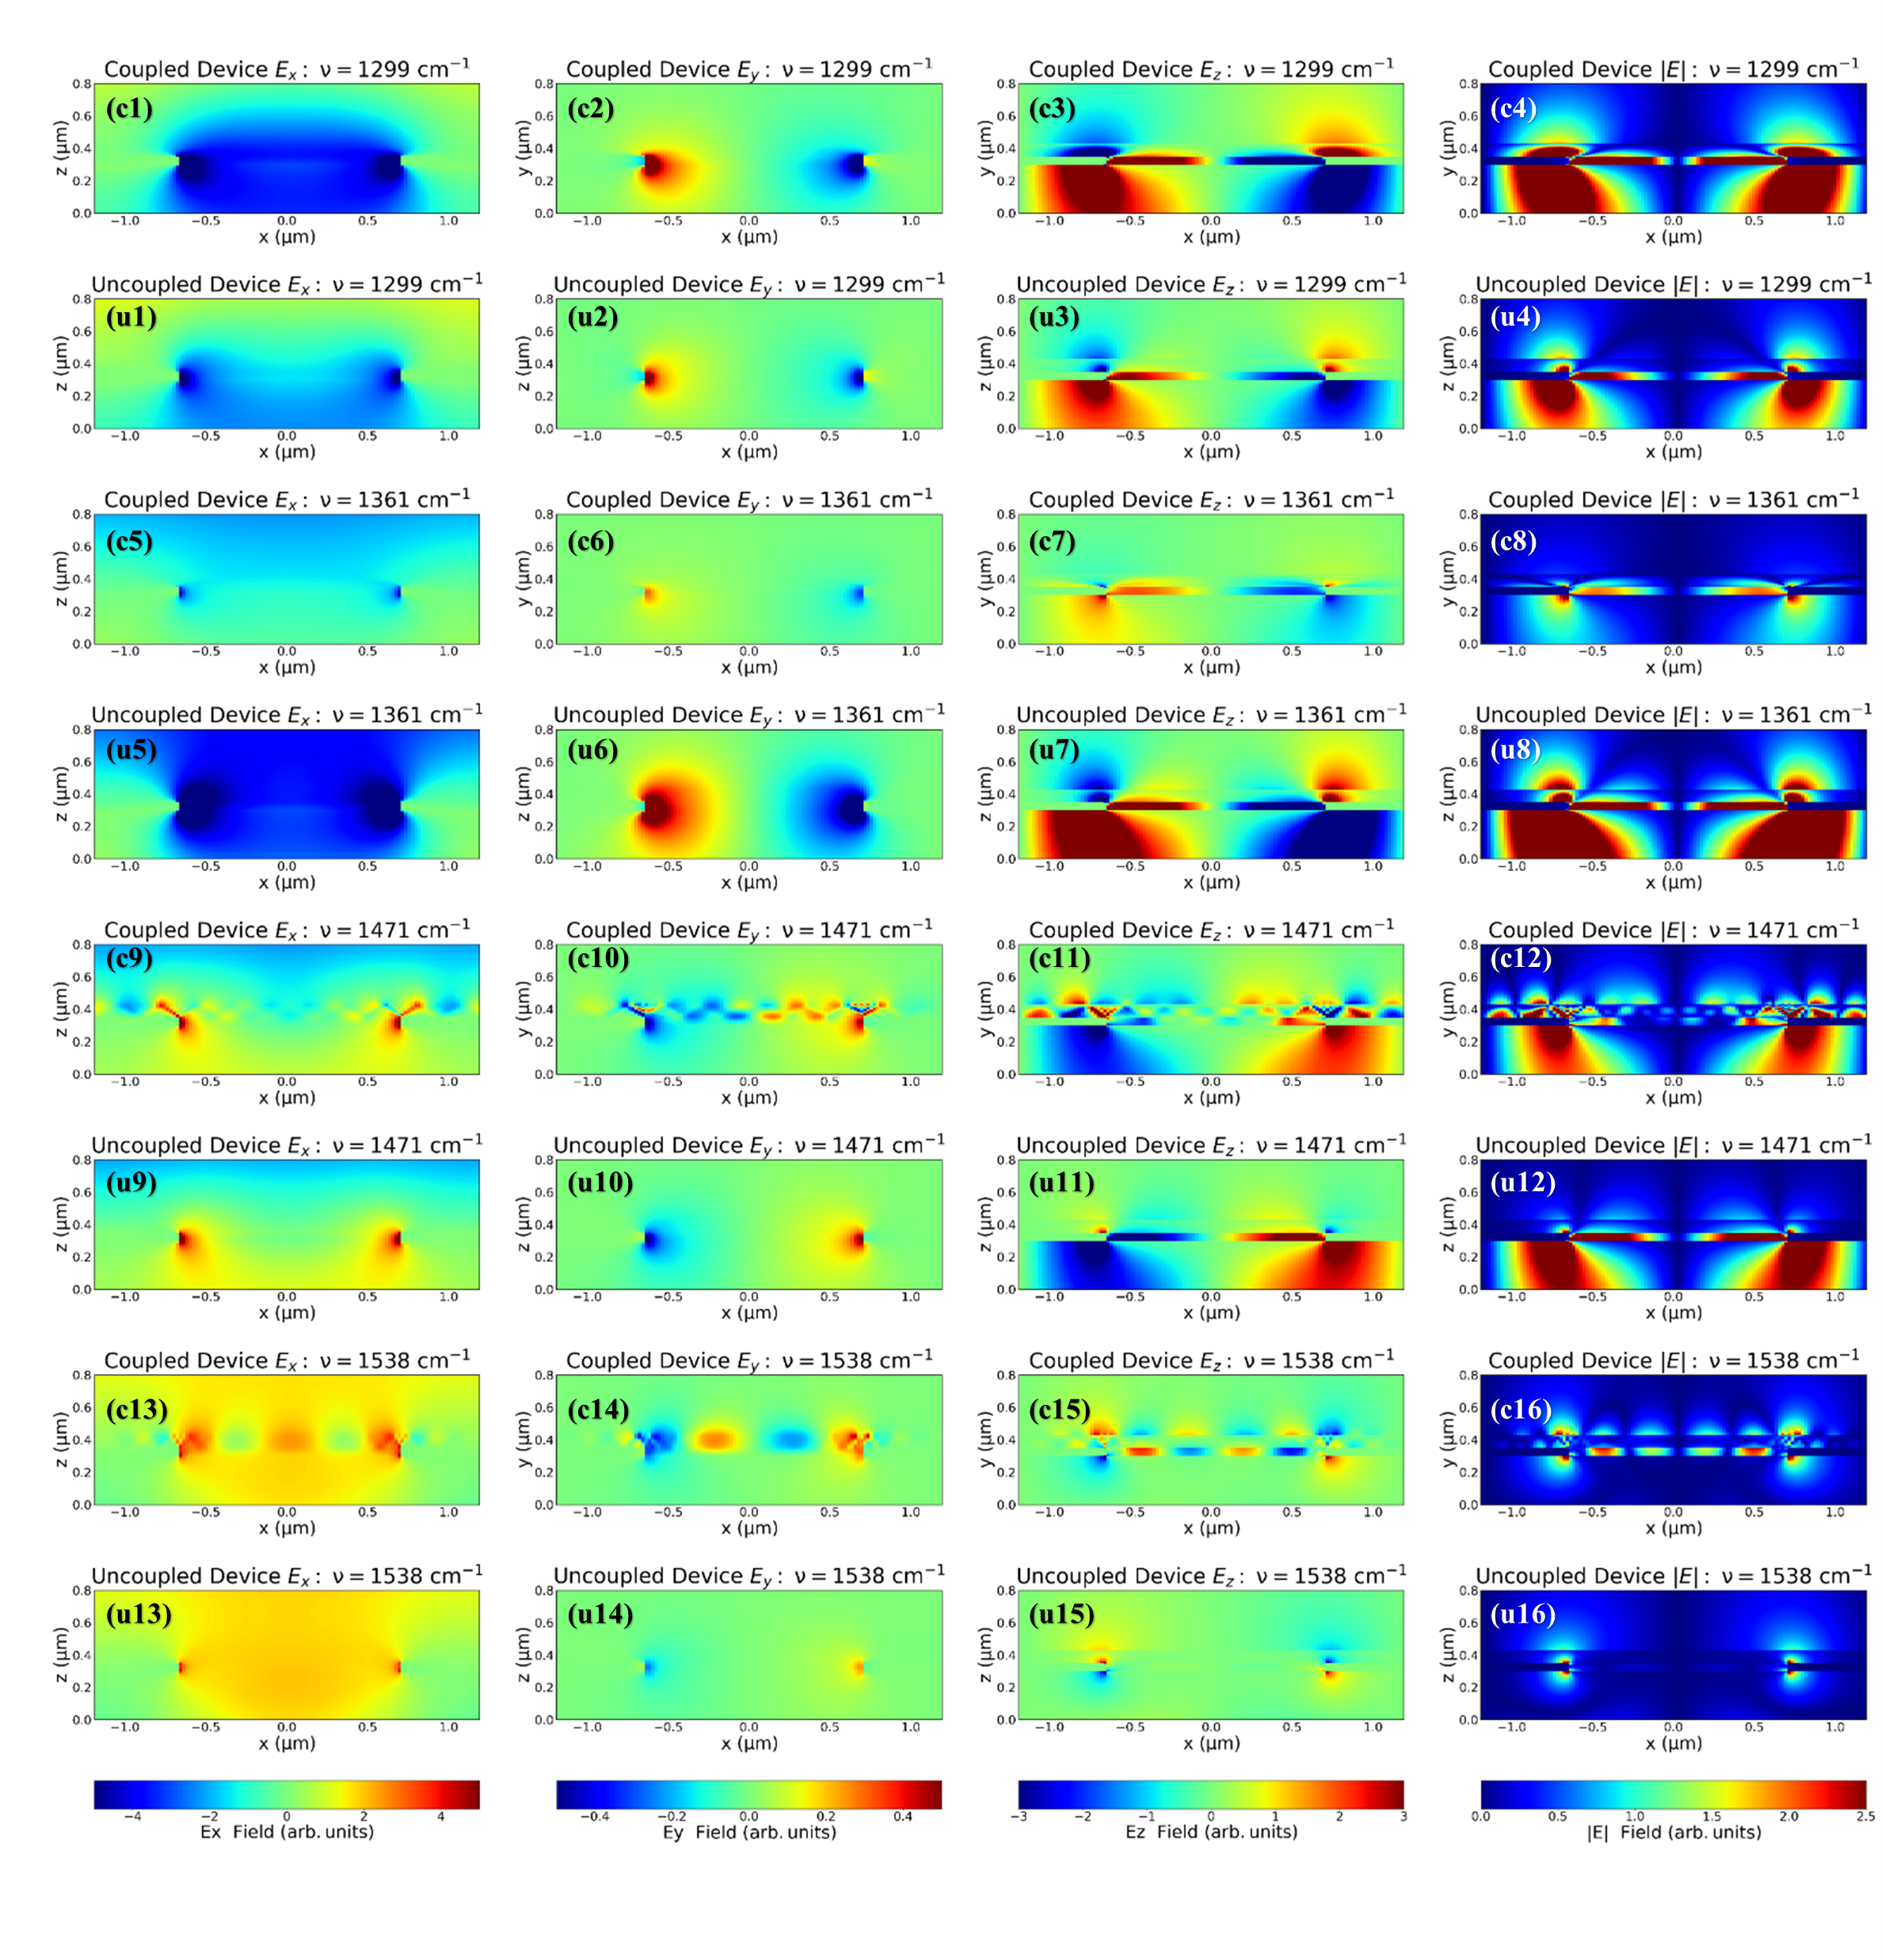
\includegraphics[width=1.0\textwidth]{FiguresCh4/Fig5.png}
        \caption{Cross-sectional colormaps of the field components in both the hBN (coupled) devices and uncoupled devices at four representative frequencies}
        \caption*{Cross-sectional colormaps of the field components in both the hBN (coupled) devices and uncoupled devices at four representative frequencies. Panes \textbf{(c1)}, \textbf{(c2)}, \textbf{(c3)}, and \textbf{(c4)} show the field in the hBN (coupled) device at monitored at 1298 $\rm cm^{-1}$. Panes \textbf{(u1)}, \textbf{(u2)}, \textbf{(u3)}, and \textbf{(u4)} show the field in the uncoupled device at the same frequency. The remaining 16 panes follow the same ordering scheme but for monitoring frequencies of 1361, 1471 and 1538 $\rm cm^{-1}$, respectively.}
        \label{fig:5}
      \end{figure}

      \begin{figure}[!htb]
        \centering\includegraphics[width=0.80\textwidth]{Mar5DisserrtationPics/Fig6Together.png}
        \caption{Experimental and simulational planar colormaps and their central lineout data.}
        \caption*{\textbf{(a)}, \textbf{(b)}, \textbf{(c)}, \textbf{(d)} and \textbf{(e)} Experimental s-SNOM images monitored at 1389, 1408, 1449, 1538 and 1562 $\rm cm^{-1}$, respectively. \textbf{(f)}, \textbf{(g)}, \textbf{(h)}, \textbf{(i)} and \textbf{(j)} Plots of the magnitude if the electric field at the vacuum/hBN interface monitored at 1266, 1408, 1449, and 1538 $\rm cm^{-1}$, respectively. (k) Line-out data from the s-SNOM data plotted as a function of position across the line indicated in \textbf{(a)} - \textbf{(e)}. \textbf{(l)}  Line-out data from the magnitude of the electric field data plotted along the line in \textbf{(f)} - \textbf{(j)}. The dashed lines in \textbf{(l)} and \textbf{(k)} represent the position of the cavity beneath the hBN layer. All data in this figure were individually scaled for greater ease of comparison.}
        \label{fig:6}
      \end{figure}

      Figure ~\ref{fig:6} presents a comparison of s-SNOM data and FDTD electric field (|\textbf{\textit{E}}|) data detected at the hBN/vacuum interface. In an examination of the s-SNOM data and the FDTD field map at 1389 $\rm cm^{-1}$, both show a bright central spot. At 1408 $\rm cm^{-1}$ data show a sharp ring feature within the Ag hole. At 1449 $\rm cm^{-1}$ the ring feature moves further out towards the edge of the Ag hole. At 1538 $\rm cm^{-1}$, there is a slow variation within the Ag hole with a weaker maximum at the center, while outside the Ag hole fine fringes can be observed which are attributed to phonon-polaritons. Finally, at 1562 $\rm cm^{-1}$, the fringes inside the Ag hole move further toward the edge of the. Outside the Ag hole fine fringes can still be observed, although they are weaker than those observed in the 1538 $\rm cm^{-1}$ case. The above behavior can also be observed by comparing the line-out data in Figure ~\ref{fig:6} (k) and (l).





  \section{Conclusion}
  \label{sec:conclusion}
    The excitations that occur on a hBN/nanopatterened Ag device have been investigated using a combination of experimental (s-SNOM) and simulational (FDTD) techniques. The s-SNOM data shows high spatial frequency features when the structure is excited in the region 1370 –1590 $\rm cm^{-1}$  and predominantly low spatial frequency features when excited outside of the spectral region. FDTD simulations of a model structure exhibit similar behavior. In addition, an examination of absorption spectra for the device indicates that the degenerate phonon and plasmon peaks split and shift enabling the phonon-plasmon coupling strength to be estimated, \textit{i.e.}, $\Delta{\rm{PP}}$ = 89.7 $\rm cm^{-1}$  to be made. Access to the individual field component afforded by the FDTD simulations enabled the polariton wavelength as function of frequency to be extracted. The results presented in this paper therefore contribute to a deeper and more fundamental understanding of the interactions between phonons and plasmons in this and related structures and devices.
  




% \input{new_bigtable_onepage.tex} %Example of a large table loaded externally
%%%%%%%%%%%%%%%%%%%%%%%%%%%%%%%%%%%%%%%%%%%%%%%%%%
%%%%%%%%%% Paper III: Paper to be submitted   %%%%%
%%%%%%%%%%%%%%%%%%%%%%%%%%%%%%%%%%%%%%%%%%%%%%%%%%
\chapter[Other Paper]
{Other Chapter%
  \footnote{D.J.T Heneghan, W. M. Dennis,2021, 
  \emph{Journal TBD}, Vol. TBD, No. TBD. \indent\indent Reprinted here with permission of publisher and authors.}}
\label{chapter:MHD}
\newpage

\section{A Yet To Be Submitted Paper}
\label{sec:intro3}



 \section{Standard section}
 
 This is a standard section

\chapter{Conclusions}
\label{chapter:dissconclusion}
Clearly your dissertation conclusions go here. 


\appendix % In case you need an appendix 

\chapter{Extra Parameters}\label{appendixextraparams}
% 
% The latex file knows to recognize the chapters after Appendix notation as letters.
% For example, this text appears in \ref{appendixextraparams}. 


%\begin{thebibliography}{1}
% You may use a different bibiography style. I've included the apj.bst file so this file compiles. This works for The Astrophysical Journal. You might publish somewhere else. Look for their .bst
% file and change things accordingly. 
\bibliographystyle{unsrt}
\bibliography{dissertation.bib}

%\end{thebibliography}

\end{document}

